\documentclass[oneside,12pt,openany]{report}

% ======================================================================
%  TIET report layout (built in, so no external tietreport.cls is needed)
% ======================================================================
\makeatletter
%% ===================================================
%% Geometry: Page margins (same on every page)
%% ===================================================
%% Equal left and right margins keep the 6in text
%% block in the same place on every page and centre
%% the title page. Top/bottom margins accommodate
%% headers/footers and content balance.
\usepackage[
  left=1.25in,
  right=1.25in,
  top=1.8in,
  bottom=0.85in
]{geometry}

%% ===================================================
%% Fancyhdr: Headers with page numbers
%% ===================================================
%% All pages: page number + course header on the
%% left. Footer empty to maximize text area.
%% Header rule (0.5pt) provides visual separation.
\usepackage{fancyhdr}
\pagestyle{fancy}
\fancyhf{}
\fancyhead[L]{\thepage \quad \@tpHeader}
\renewcommand{\headrulewidth}{0.5pt}
\renewcommand{\footrulewidth}{0pt}

%% ===================================================
%% Titlesec: Custom chapter title formatting
%% ===================================================
%% Chapter titles use raggedleft (right-aligned)
%% with bold/large label, followed by huge title
%% and horizontal rule. Spacing optimized for
%% visual hierarchy. Chapter opening pages use
%% empty style (no headers).
\usepackage{titlesec}
\titleformat{\chapter}[display]
  {\raggedleft\bfseries\large}
  {Chapter \thechapter}
  {0.3em}
  {\huge}
  [\vspace{0.1em}\hrule]
\titlespacing*{\chapter}{0pt}{-50pt}{40pt}
\assignpagestyle{\chapter}{empty}

%% ===================================================
%% Required packages: Hyperref, graphics, math
%% ===================================================
%% Standard packages for links, images, and
%% mathematical notation support.
\usepackage{hyperref}
\usepackage{graphicx}
\usepackage{amsmath}
\usepackage{amssymb}

%% ===================================================
%% Internal Variables: Title page content storage
%% ===================================================
%% Prefix @tp denotes "title page" internal vars.
%% These hold configuration set via public commands
%% below. Users should not access these directly.

%% Title page header (e.g., course code and lab)
\newcommand{\@tpHeader}{%
  UCS 503 Software Engineering Project Report%
}

%% Main project title
\newcommand{\@tpTitle}{Proposal to Final}

%% Project subtitle/description
\newcommand{\@tpSubTitle}{%
  How to Write a Project Report%
}

%% Author list (4 students with roll numbers)
\newcommand{\@tpAuthors}{%
  \texttt{102XXXXXXX} {Name Title} \\
  \texttt{102XXXXXXX} {Name Title} \\
  \texttt{102XXXXXXX} {Name Title} \\
  \texttt{102XXXXXXX} {Name Title}%
}

%% Degree, year, group info below authors
\newcommand{\@tpSubText}{%
  Group: \texttt{3XXX} BE Third Year, CSE%
}

%% Faculty advisor/guide name
\newcommand{\@tpAdvisor}{%
  Dr. NAME OF THE ADVISOR%
}

%% Footer: evaluation period, department, institution
\newcommand{\@tpFooter}{%
  \large Mid-Semester Evaluation \\[0.2cm]
  \bfseries Computer Science and Engineering%
  \\ Department \\[0.15cm]
  Thapar Institute of Engineering and%
  \\ Technology, Patiala%
}

%% ===================================================
%% Public Commands: User-facing configuration
%% ===================================================
%% Call these in preamble to customize title page.
%% Example: \TitlePageHeader{CS 504 Lab}

%% Set title page header
\newcommand{\TitlePageHeader}[1]{%
  \renewcommand{\@tpHeader}{#1}%
}

%% Set main project title
\newcommand{\ProjectTitle}[1]{%
  \renewcommand{\@tpTitle}{#1}%
}

%% Set project subtitle
\newcommand{\ProjectSubTitle}[1]{%
  \renewcommand{\@tpSubTitle}{#1}%
}

%% Set author list (override default)
\renewcommand{\author}[1]{%
  \renewcommand{\@tpAuthors}{#1}%
}

%% Set degree/year/group info
\newcommand{\TitlePageSubText}[1]{%
  \renewcommand{\@tpSubText}{#1}%
}

%% Set advisor name
\newcommand{\AdvisorName}[1]{%
  \renewcommand{\@tpAdvisor}{#1}%
}

%% Set footer text (evaluation period, dept, etc)
\newcommand{\TitlePageFooterText}[1]{%
  \renewcommand{\@tpFooter}{#1}%
}

%% ===================================================
%% Maketitle: Render custom title page
%% ===================================================
%% Override \maketitle to produce styled title page
%% using configured variables. Centered layout with
%% institutional branding. After title page, a blank
%% page follows (ready for TOC on next page).

\renewcommand{\maketitle}{%
  \begin{titlepage}
    \thispagestyle{empty}
    \centering
    \vspace*{0.5cm}

    {\large \textbf{\@tpHeader}}

    \vspace{2cm}
    {\LARGE \textbf{\@tpTitle}}

    \vspace{0.2cm}
    {\@tpSubTitle}

    \vspace{3.5cm}
    {\large \textbf{Submitted by:}}

    \vspace{0.2cm}
    {\large \@tpAuthors}

    \vspace{0.5cm}
    {\normalsize \@tpSubText}

    \vfill

    {\large \textbf{Submitted to:}}

    \vspace{0.2cm}
    {\normalsize \@tpAdvisor}

    \vspace{2cm}
    {\normalsize \@tpFooter}
  \end{titlepage}

  \newpage
  \thispagestyle{empty}%
}
\makeatother



% Extra packages required by the report content
\usepackage{float}
\usepackage{tabularx}
\usepackage{xcolor}
\usepackage{listings}
\usepackage{adjustbox}
\usepackage{needspace}
\usepackage{tikz}
\usetikzlibrary{arrows.meta,positioning,shapes.geometric,fit,calc}



%% ==================================================
%% CODE LISTING AND DIAGRAM STYLES
%% ==================================================

\lstdefinestyle{code}{
  basicstyle=\ttfamily\scriptsize,
  keywordstyle=\bfseries,
  commentstyle=\color{gray}\itshape,
  numbers=left, numberstyle=\tiny\color{gray}, numbersep=5pt,
  frame=single, rulecolor=\color{gray!60},
  backgroundcolor=\color{gray!6},
  breaklines=true, tabsize=2, showstringspaces=false,
  xleftmargin=1.2em, aboveskip=4pt, belowskip=2pt
}
\lstdefinelanguage{json}{
  string=[b]", morekeywords={true,false}, sensitive=true
}

\tikzset{
  >=Stealth,
  blk/.style={rectangle,rounded corners=3pt,draw=black,fill=white,thick,
              minimum height=1.2cm,text width=2.3cm,align=center,font=\small},
  fl/.style={font=\scriptsize,align=center}
}

% ground symbol: \gnd{coordinate}
\newcommand{\gnd}[1]{%
  \draw[thick] (#1) -- ++(0,-0.3) coordinate (g);
  \draw[thick] ($(g)+(-0.25,0)$) -- ($(g)+(0.25,0)$);
  \draw[thick] ($(g)+(-0.16,-0.08)$) -- ($(g)+(0.16,-0.08)$);
  \draw[thick] ($(g)+(-0.07,-0.16)$) -- ($(g)+(0.07,-0.16)$);}

% UML stick-figure actor: \actor{x}{y}{label}
\newcommand{\actor}[3]{%
  \begin{scope}[shift={(#1,#2)}]
    \draw[thick] (0,0.55) circle (0.17);
    \draw[thick] (0,0.38)--(0,-0.1) (-0.3,0.25)--(0.3,0.25)
                 (0,-0.1)--(-0.25,-0.5) (0,-0.1)--(0.25,-0.5);
    \node[font=\footnotesize,align=center,below] at (0,-0.5) {#3};
  \end{scope}}

% Scale a diagram down only if it is wider/taller than the page allows
\newcommand{\fitfig}[2][0.27]{\begin{adjustbox}{max width=\linewidth,max height=#1\textheight,center}#2\end{adjustbox}}

%% ==================================================
%% CUSTOMIZE THESE FIELDS FOR YOUR PROJECT
%% ==================================================

% Course/Lab header
\TitlePageHeader{%
  UCS 503 - Software Engineering%
}

% Main project title
\ProjectTitle{%
  SmartLib: Library Seat Allocator%
}

% Subtitle or project description
\ProjectSubTitle{%
  An IoT System for Real-Time Seat Monitoring and Management%
}

% Student information (up to 4 students)
\author{%
  \texttt{1024031135} Saksham Kansal \\
  \texttt{1024031118} Ishaan Gupta \\
  \texttt{1024031137} Sanshi%
}

% Group number, degree, year, program
\TitlePageSubText{%
  Computer Engineering Department (COE)%
}

% Faculty advisor/guide name
\AdvisorName{%
  Ms. Jhonsy Bansal%
}

% Evaluation period and department info
\TitlePageFooterText{{%
    \large August 2026 \\[0.2cm]
    \bfseries Computer Engineering
    Department%
  } \\[0.15cm]
  Thapar Institute of Engineering and Technology,
  Patiala%
}

%% ==================================================

\begin{document}

% Let partly filled pages end early instead of stretching the spacing
\raggedbottom

% Generate title page
\maketitle

% Table of contents (auto-generated from chapters)
\tableofcontents

% ===== CHAPTER 1: INTRODUCTION =====

\chapter{Introduction}

\section{Background and Context}

University libraries are busiest during exams and assignment deadlines. At these times,
users have to walk through the reading halls to find a free seat. Gate counters show how many
people are inside, but not \emph{where} the free seats are. This wastes time and creates noise
that disturbs people who are studying.

Low-cost Wi-Fi boards, simple sensors and real-time cloud databases now make it possible to
track every seat and show its status on any phone or screen within a second.

\subsection{Problem Statement}
\label{sec:problem}

Finding a seat today has three main problems, listed in Table~\ref{tab:problems}.

\begin{table}[H]
\centering
\small
\renewcommand{\arraystretch}{1.1}
\begin{tabularx}{\linewidth}{|>{\raggedright\arraybackslash}p{0.2\linewidth}|>{\raggedright\arraybackslash}X|>{\raggedright\arraybackslash}p{0.27\linewidth}|}
  \hline
  \textbf{Problem} & \textbf{Description} & \textbf{What is needed} \\
  \hline
  Manual search &
  Users walk across floors and aisles at busy times, which wastes time and creates noise. &
  A way to see free seats before walking to the hall. \\
  \hline
  No seat-level view &
  Headcount boards at the gate show only a total count, not which desks are free. &
  Status of each seat instead of one building-wide number. \\
  \hline
  No data for staff &
  Staff have no live or past usage data to spread users across halls or plan facilities
  such as cooling. &
  Live and past usage reports for planning. \\
  \hline
\end{tabularx}
\caption{Main problems and what is needed}
\label{tab:problems}
\end{table}

\section{Project Objectives}

\begin{enumerate}
  \item \textbf{Detection:} Detect whether each seat is in use with low-cost IR sensors.
  \item \textbf{Noise filtering:} Ignore short disturbances, such as a passing hand, so a
    seat's status does not flicker.
  \item \textbf{Transmission:} Send seat status to the cloud over Wi-Fi with little delay.
  \item \textbf{User view:} Show a live seat map and seat counts on phones and on a screen at
    the entrance.
  \item \textbf{Admin view:} Give staff a dashboard with usage, session time and busy hours.
\end{enumerate}

\subsection{Scope and Organisation of the Report}

The system covers sensing, sending, storing and displaying seat status for one library zone.
It only detects whether a seat is in use. It does not take pictures, identify people or handle
seat bookings. The prototype shows the full path from a sensor to a web browser, and more
seats or zones can be added with more sensor nodes and database entries.

Chapter~\ref{ch:method} covers the requirements, development model, design, diagrams and
implementation. Chapter~\ref{ch:results} gives the test plan and limitations, and
Chapter~\ref{ch:concl} concludes with future work.

% ===== CHAPTER 2: METHODOLOGY & DESIGN =====

\chapter{Methodology and Design}
\label{ch:method}

\section{Requirements Analysis}
\label{sec:req}

\subsection{Stakeholders}

\begin{itemize}
  \item \textbf{Users:} Want to know which seats are free and how full the library is.
  \item \textbf{Library staff / administrators:} Want live and past usage data to manage
    the library.
  \item \textbf{Sensor node (system actor):} Checks each seat and sends its status.
\end{itemize}

\subsection{Functional Requirements}

\begin{table}[H]
\centering
\small
\renewcommand{\arraystretch}{1.1}
\begin{tabularx}{\linewidth}{|l|>{\raggedright\arraybackslash}X|}
  \hline
  \textbf{ID} & \textbf{Requirement} \\
  \hline
  FR1 & Detect whether a person is at each seat using an IR sensor. \\
  \hline
  FR2 & Change a seat's status only after the new reading stays the same for 3~seconds
        (debounce). \\
  \hline
  FR3 & The ESP32 sends seat status as JSON over Wi-Fi to the cloud database. \\
  \hline
  FR4 & The database stores the latest status and updates all screens without a page
        refresh. \\
  \hline
  FR5 & The user dashboard shows a seat map: free seats in green, taken seats in red. \\
  \hline
  FR6 & The dashboards show total, taken and free seats, and the percentage in use. \\
  \hline
  FR7 & The entrance screen shows live seat availability for the zone. \\
  \hline
  FR8 & The admin dashboard shows average session time, busiest hour, weekly trend, hourly
        usage and the taken/free split. \\
  \hline
\end{tabularx}
\caption{Functional requirements}
\label{tab:fr}
\end{table}

\subsection{Non-Functional Requirements}

\begin{table}[H]
\centering
\small
\renewcommand{\arraystretch}{1.1}
\begin{tabularx}{\linewidth}{|l|l|>{\raggedright\arraybackslash}X|}
  \hline
  \textbf{ID} & \textbf{Attribute} & \textbf{Requirement} \\
  \hline
  NFR1 & Performance & Screens update within one second of a database change (not counting
                       the 3-second debounce). \\
  \hline
  NFR2 & Reliability & Short disturbances must not make seat colours flicker. \\
  \hline
  NFR3 & Usability   & The user interface works well on a phone browser. \\
  \hline
  NFR4 & Scalability & New seats and zones can be added without changing the design. \\
  \hline
  NFR5 & Cost        & Uses cheap, easily available hardware. \\
  \hline
  NFR6 & Privacy     & No images or personal data; only ``in use'' or ``free'' is stored. \\
  \hline
\end{tabularx}
\caption{Non-functional requirements}
\label{tab:nfr}
\end{table}

\section{Software Development Process Model}
\label{sec:process}

The project follows the \emph{Incremental Development Model}~\cite{sommerville,pressman}.
The requirements in Section~\ref{sec:req} are set first. The system is then built in parts
(increments). Each part is designed, built and tested, then joined to the parts already
finished, so every stage ends with something that works (Figure~\ref{fig:process}).

\begin{figure}[H]
\centering
\fitfig[0.3]{%
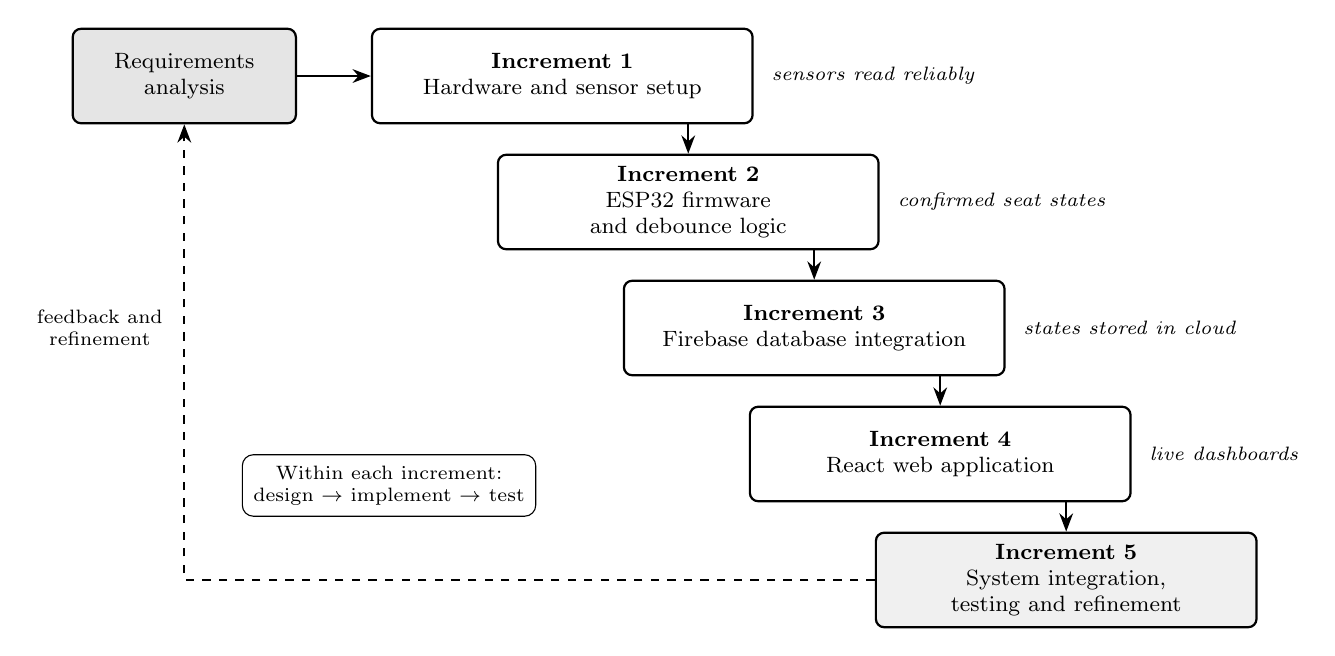
\begin{tikzpicture}[
  req/.style={rectangle,rounded corners=3pt,draw,thick,fill=gray!20,minimum height=1.2cm,
              text width=2.6cm,align=center,font=\footnotesize},
  inc/.style={rectangle,rounded corners=3pt,draw,thick,fill=white,minimum height=1.2cm,
              text width=4.6cm,align=center,font=\footnotesize},
  incout/.style={font=\scriptsize\itshape,align=left,anchor=west}]
  \node[req] (r)  at (0,0) {Requirements\\analysis};
  \node[inc] (i1) at (4.8,0)     {\textbf{Increment 1}\\Hardware and sensor setup};
  \node[inc] (i2) at (6.4,-1.6)  {\textbf{Increment 2}\\ESP32 firmware and debounce logic};
  \node[inc] (i3) at (8.0,-3.2)  {\textbf{Increment 3}\\Firebase database integration};
  \node[inc] (i4) at (9.6,-4.8)  {\textbf{Increment 4}\\React web application};
  \node[inc,fill=gray!12] (i5) at (11.2,-6.4) {\textbf{Increment 5}\\System integration,
                                               testing and refinement};
  \draw[->,thick] (r) -- (i1);
  \draw[->,thick] (i2.north |- i1.south) -- (i2.north);
  \draw[->,thick] (i3.north |- i2.south) -- (i3.north);
  \draw[->,thick] (i4.north |- i3.south) -- (i4.north);
  \draw[->,thick] (i5.north |- i4.south) -- (i5.north);
  \node[incout] at ([xshift=3pt]i1.east) {sensors read reliably};
  \node[incout] at ([xshift=3pt]i2.east) {confirmed seat states};
  \node[incout] at ([xshift=3pt]i3.east) {states stored in cloud};
  \node[incout] at ([xshift=3pt]i4.east) {live dashboards};
  \draw[->,thick,dashed] (i5.west) -| (r.south);
  \node[fl,anchor=east] at (-0.15,-3.2) {feedback and\\refinement};
  \node[draw,rounded corners,font=\scriptsize,align=center,inner sep=4pt] at (2.6,-5.2)
       {Within each increment:\\design $\rightarrow$ implement $\rightarrow$ test};
\end{tikzpicture}}
\caption{Incremental development model for the Library Seat Allocator}
\label{fig:process}
\end{figure}

Increment 1 fits the IR sensors to the ESP32 and checks their output at each seat.
Increment 2 adds sensor reading and the 3-second debounce (FR1, FR2). Increment 3 sends the
seat status to Firebase as JSON (FR3, FR4). Increment 4 builds the user dashboard, admin
dashboard and entrance screen (FR5--FR8). Increment 5 joins everything and tests it with the
cases in Chapter~\ref{ch:results}; any problems are fixed in the earlier parts.

\textbf{Why this model.} The project has hardware, firmware, a cloud database and a web app,
and each part depends on the one before it. Building them one at a time lets each part be
tested on its own, so a fault is easy to locate. Each increment also gives a working result
that can be shown, and later parts can change without starting over.

\section{System Architecture}

\subsection{High-Level Design}

The system has three layers (Figure~\ref{fig:arch}): the \emph{edge layer} senses the seats,
the \emph{cloud layer} stores and shares their status, and the \emph{presentation layer}
shows it to users and staff.

\begin{figure}[H]
\centering
\fitfig{%
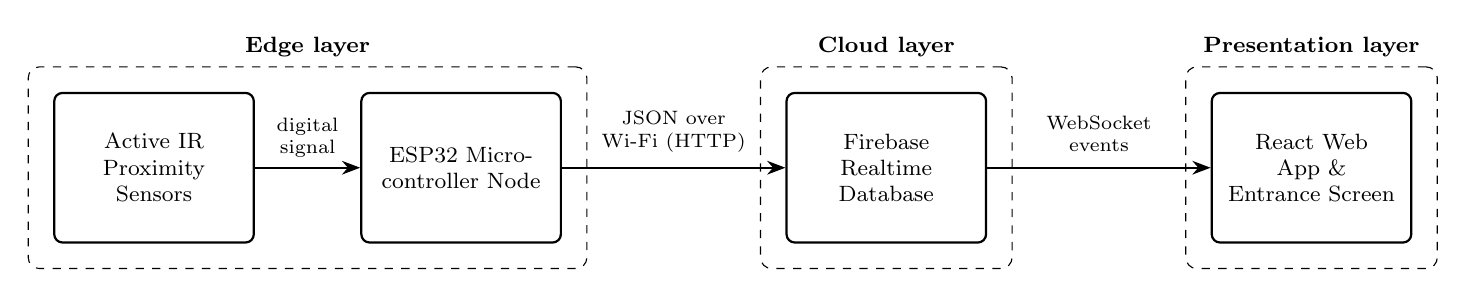
\begin{tikzpicture}[blk/.append style={text width=2.3cm,minimum height=1.9cm,font=\footnotesize}]
  \node[blk] (ir)  at (0,0)    {Active IR\\Proximity Sensors};
  \node[blk] (esp) at (3.9,0)  {ESP32 Micro-controller Node};
  \node[blk] (fb)  at (9.3,0)  {Firebase\\Realtime Database};
  \node[blk] (web) at (14.7,0) {React Web App \&\\Entrance Screen};
  \node[draw=black,dashed,rounded corners,fit=(ir)(esp),inner sep=9pt,
        label={[font=\footnotesize\bfseries,text=black]above:Edge layer}] (edge) {};
  \node[draw=black,dashed,rounded corners,fit=(fb),inner sep=9pt,
        label={[font=\footnotesize\bfseries,text=black]above:Cloud layer}] (cloud) {};
  \node[draw=black,dashed,rounded corners,fit=(web),inner sep=9pt,
        label={[font=\footnotesize\bfseries,text=black]above:Presentation layer}] (pres) {};
  \draw[->,thick] (ir)  -- node[fl,above]{digital\\signal} (esp);
  \draw[->,thick] (esp) -- node[fl,above=2pt]{JSON over\\Wi-Fi (HTTP)} (fb);
  \draw[->,thick] (fb)  -- node[fl,above=2pt]{WebSocket\\events} (web);
\end{tikzpicture}}
\caption{End-to-end system architecture}
\label{fig:arch}
\end{figure}

The IR sensors send signals to the ESP32~\cite{esp32}, which sends the confirmed seat status
as JSON over Wi-Fi to the Firebase Realtime Database~\cite{firebase}. The database then pushes
each change to the React web app and the entrance screen~\cite{react}.

\subsection{Seating Layout}

Figure~\ref{fig:seating} shows the seat arrangement. Each seat has an IR sensor at the table
edge, facing the chair. The sensors are wired to a controller linked to the ESP32. In the
figure, a free seat is white and a taken seat is dark; the dashboards use green and red.

\begin{figure}[H]
\centering
\fitfig{%
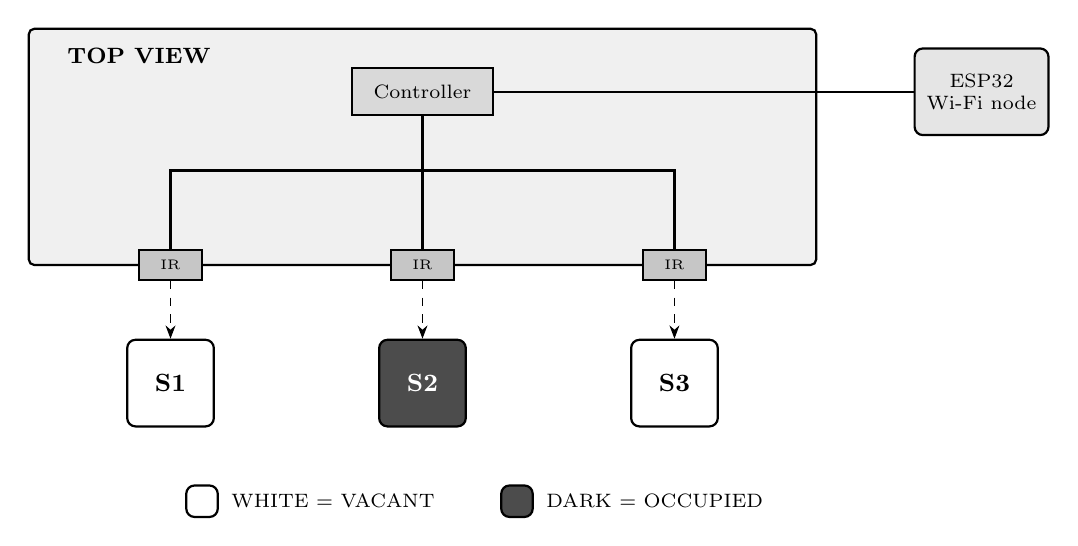
\begin{tikzpicture}[
  seat/.style={draw=black,fill=#1,thick,rounded corners=3pt,minimum size=1.1cm,font=\small\bfseries},
  irn/.style={draw,thick,fill=gray!45,minimum width=0.8cm,minimum height=0.38cm,font=\tiny}]
  \draw[thick,fill=gray!12,rounded corners=2pt] (0,0) rectangle (10,3);
  \node[font=\footnotesize\bfseries] at (1.4,2.65) {TOP VIEW};
  \node[draw,thick,fill=gray!30,minimum width=1.8cm,minimum height=0.6cm,font=\scriptsize] (ctl) at (5,2.2) {Controller};
  \foreach \x/\n in {1.8/1,5/2,8.2/3}{
    \node[irn] (ir\n) at (\x,0) {IR};
  }
  \coordinate (j) at (5,1.2);
  \draw[thick] (ctl.south) -- (j);
  \draw[thick] (j) -| (ir1.north);
  \draw[thick] (j) -- (ir2.north);
  \draw[thick] (j) -| (ir3.north);
  \node[seat=white] (c1) at (1.8,-1.5) {S1};
  \node[seat=black!70,text=white] (c2) at (5.0,-1.5) {S2};
  \node[seat=white] (c3) at (8.2,-1.5) {S3};
  \foreach \n in {1,2,3}{ \draw[dashed,->] (ir\n.south) -- (c\n.north); }
  \node[draw,thick,fill=gray!20,rounded corners=3pt,minimum width=1.7cm,minimum height=1.1cm,
        font=\scriptsize,align=center] (wifi) at (12.1,2.2) {ESP32\\Wi-Fi node};
  \draw[thick] (ctl.east) -- (wifi.west);
  \node[seat=white,minimum size=0.4cm] at (2.2,-3.0) {};
  \node[font=\scriptsize,right] at (2.45,-3.0) {WHITE = VACANT};
  \node[seat=black!70,minimum size=0.4cm] at (6.2,-3.0) {};
  \node[font=\scriptsize,right] at (6.45,-3.0) {DARK = OCCUPIED};
\end{tikzpicture}}
\caption{Seating layout (top view): per-seat IR sensors wired to a controller and an ESP32 node}
\label{fig:seating}
\end{figure}

\subsection{Technical Stack}
\label{sec:stack}

\begin{itemize}
  \item \textbf{Hardware:} ESP32 development board~\cite{esp32}; one IR proximity sensor per
    seat (GPIO~27 and GPIO~28 in the prototype); two push buttons on GPIO~18 and GPIO~19;
    a 5\,V power supply; perforated board and jumper wires.
  \item \textbf{Framework/Language:} C++ with the Arduino framework for the ESP32 firmware;
    React with JavaScript for the web app~\cite{react}.
  \item \textbf{Database:} Firebase Realtime Database~\cite{firebase}. Seat status is kept
    as JSON under \texttt{library/zone1}, with one entry per seat (\texttt{s1},
    \texttt{s2}, \ldots) holding a true/false \texttt{occupied} value.
  \item \textbf{Libraries:} the ESP32 \texttt{WiFi} and \texttt{HTTPClient} libraries for
    sending data; the Firebase SDK in the web app for live updates; SVG for drawing the
    seat map.
  \item \textbf{Tools:} an Arduino-compatible IDE to build and upload the firmware; a web
    browser on a laptop and a phone for testing the dashboards.
\end{itemize}

\section{System Modeling Diagrams}
\label{sec:models}

Each diagram shows the system from a different angle: who uses it (use case), how data
moves (DFDs), what happens over time (sequence diagram and state machine) and the order of
steps in the firmware (flowchart).

\subsection{Use Case Diagram}

Figure~\ref{fig:usecase} shows who uses the system and how~\cite{uml}. Users view the seat
map and availability, staff view the reports, and the sensor node detects seats and sends
their status.

\begin{figure}[H]
\centering
\fitfig[0.42]{%
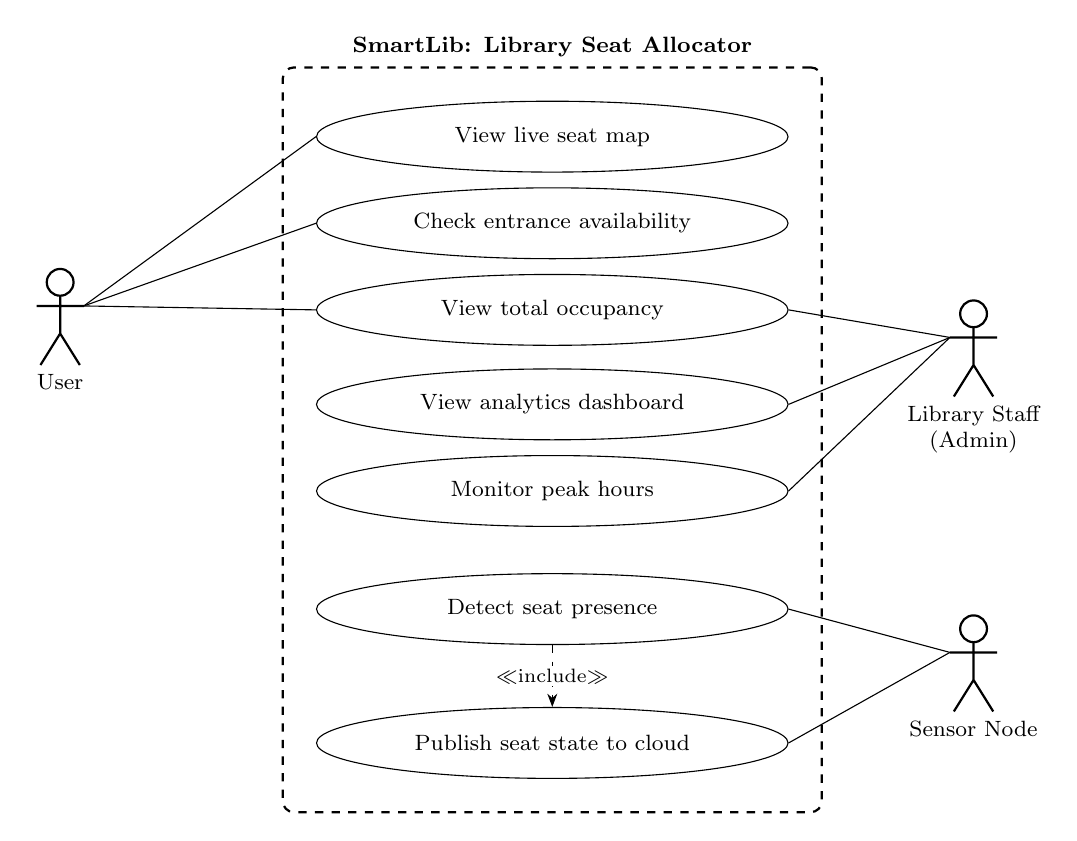
\begin{tikzpicture}[
  uc/.style={ellipse,draw,fill=white,minimum height=0.9cm,text width=4.0cm,align=center,font=\footnotesize}]
  \node[uc] (uc1) at (6.25,3.4)  {View live seat map};
  \node[uc] (uc2) at (6.25,2.3)  {Check entrance availability};
  \node[uc] (uc3) at (6.25,1.2)  {View total occupancy};
  \node[uc] (uc4) at (6.25,0)    {View analytics dashboard};
  \node[uc] (uc5) at (6.25,-1.1) {Monitor peak hours};
  \node[uc] (uc6) at (6.25,-2.6) {Detect seat presence};
  \node[uc] (uc7) at (6.25,-4.3) {Publish seat state to cloud};
  \node[draw,thick,dashed,rounded corners,fit=(uc1)(uc2)(uc3)(uc4)(uc5)(uc6)(uc7),inner sep=12pt,
        label={[font=\footnotesize\bfseries]above:SmartLib: Library Seat Allocator}] (sys) {};
  \actor{0}{1.0}{User}
  \actor{11.6}{0.6}{Library Staff\\(Admin)}
  \actor{11.6}{-3.4}{Sensor Node}
  \draw (0.3,1.25) -- (uc1.west);
  \draw (0.3,1.25) -- (uc2.west);
  \draw (0.3,1.25) -- (uc3.west);
  \draw (11.3,0.85) -- (uc3.east);
  \draw (11.3,0.85) -- (uc4.east);
  \draw (11.3,0.85) -- (uc5.east);
  \draw (11.3,-3.15) -- (uc6.east);
  \draw (11.3,-3.15) -- (uc7.east);
  \draw[->,dashed] (uc6) -- node[fill=white,inner sep=1pt,font=\scriptsize]{$\ll$include$\gg$} (uc7);
\end{tikzpicture}}
\caption{Use case diagram}
\label{fig:usecase}
\end{figure}

\subsection{Data Flow Diagrams}

The level-0 diagram (Figure~\ref{fig:dfd0}) shows the whole system as one process. The
level-1 diagram (Figure~\ref{fig:dfd1}) splits it into four processes and one data store.

\begin{figure}[H]
\centering
\fitfig[0.27]{%
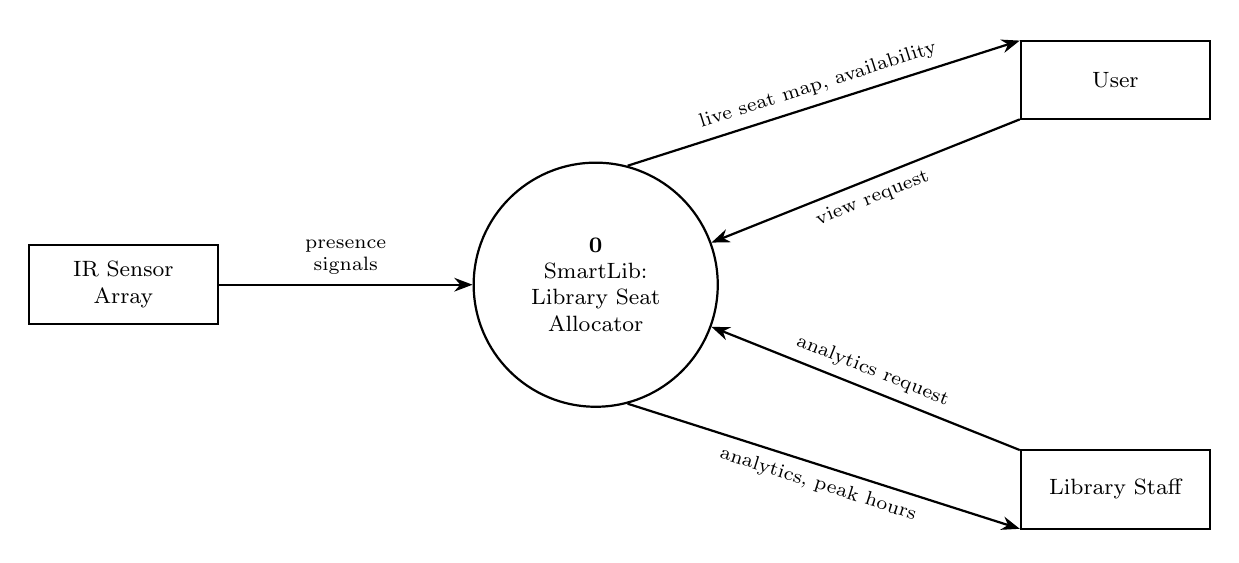
\begin{tikzpicture}[
  ent/.style={rectangle,draw,thick,fill=white,minimum width=2.4cm,minimum height=1cm,align=center,font=\footnotesize},
  proc/.style={circle,draw,thick,fill=white,minimum size=3.1cm,align=center,font=\footnotesize}]
  \node[ent]  (sens) at (0,0) {IR Sensor\\Array};
  \node[proc] (sys)  at (6,0) {\textbf{0}\\SmartLib:\\Library Seat\\Allocator};
  \node[ent]  (stud) at (12.6,2.6)  {User};
  \node[ent]  (adm)  at (12.6,-2.6) {Library Staff};
  \draw[->,thick] (sens) -- node[fl,above]{presence\\signals} (sys);
  \draw[->,thick] (sys.75) -- node[fl,above,sloped]{live seat map, availability} ([yshift=5mm]stud.west);
  \draw[->,thick] ([yshift=-5mm]stud.west) -- node[fl,below,sloped]{view request} (sys.20);
  \draw[->,thick] (sys.-75) -- node[fl,below,sloped]{analytics, peak hours} ([yshift=-5mm]adm.west);
  \draw[->,thick] ([yshift=5mm]adm.west) -- node[fl,above,sloped]{analytics request} (sys.-20);
\end{tikzpicture}}
\caption{Data flow diagram -- level 0 (context diagram)}
\label{fig:dfd0}
\end{figure}

\begin{figure}[H]
\centering
\fitfig[0.36]{%
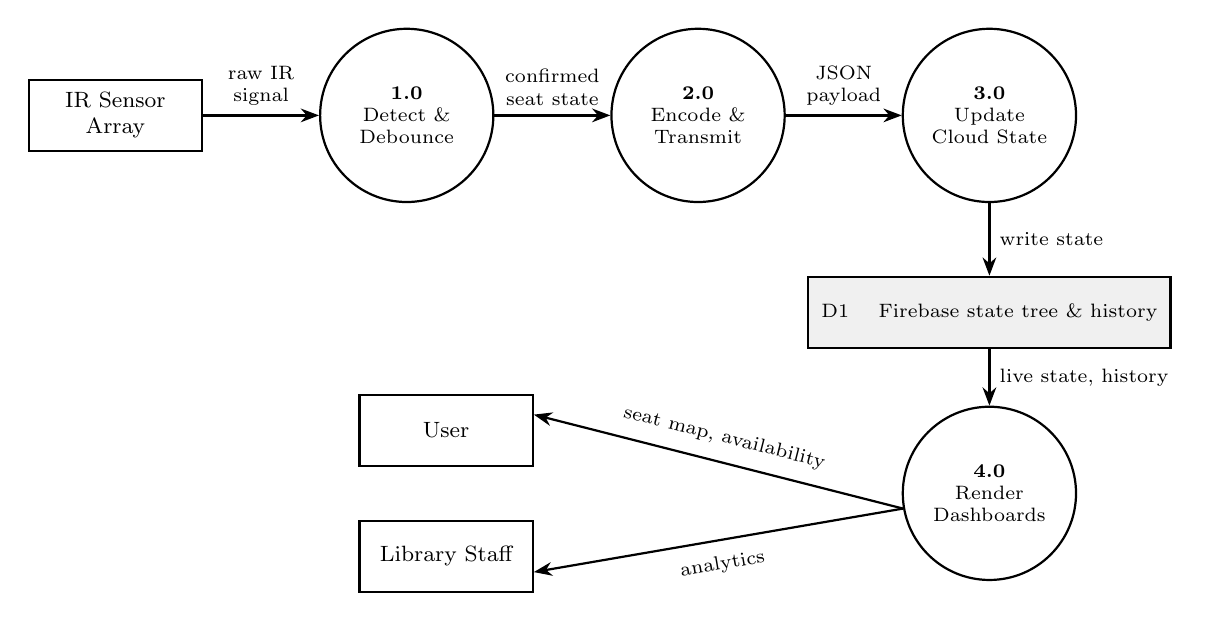
\begin{tikzpicture}[
  ent/.style={rectangle,draw,thick,fill=white,minimum width=2.2cm,minimum height=0.9cm,align=center,font=\footnotesize},
  proc/.style={circle,draw,thick,fill=white,minimum size=2.2cm,align=center,font=\scriptsize},
  store/.style={rectangle,draw,thick,fill=gray!12,minimum width=4.6cm,minimum height=0.9cm,align=center,font=\scriptsize}]
  \node[ent]  (sens) at (0,0)    {IR Sensor\\Array};
  \node[proc] (p1)   at (3.7,0)  {\textbf{1.0}\\Detect \&\\Debounce};
  \node[proc] (p2)   at (7.4,0)  {\textbf{2.0}\\Encode \&\\Transmit};
  \node[proc] (p3)   at (11.1,0) {\textbf{3.0}\\Update\\Cloud State};
  \node[store](d1)   at (11.1,-2.5) {D1 \quad Firebase state tree \& history};
  \node[proc] (p4)   at (11.1,-4.8) {\textbf{4.0}\\Render\\Dashboards};
  \node[ent]  (stud) at (4.2,-4.0)  {User};
  \node[ent]  (adm)  at (4.2,-5.6)  {Library Staff};
  \draw[->,thick] (sens) -- node[fl,above]{raw IR\\signal} (p1);
  \draw[->,thick] (p1) -- node[fl,above]{confirmed\\seat state} (p2);
  \draw[->,thick] (p2) -- node[fl,above]{JSON\\payload} (p3);
  \draw[->,thick] (p3) -- node[fl,right]{write state} (d1);
  \draw[->,thick] (d1) -- node[fl,right]{live state, history} (p4);
  \draw[->,thick] (p4.190) -- node[fl,above=2pt,sloped]{seat map, availability} ([yshift=2mm]stud.east);
  \draw[->,thick] (p4.-170) -- node[fl,below=2pt,sloped]{analytics} ([yshift=-2mm]adm.east);
\end{tikzpicture}}
\caption{Data flow diagram -- level 1}
\label{fig:dfd1}
\end{figure}

\subsection{Sequence Diagram}

Figure~\ref{fig:seq} follows one event, from a user sitting down to the seat turning red on
every dashboard. The ESP32 sends the update only after the reading stays the same for
3~seconds.

\begin{figure}[H]
\centering
\fitfig[0.36]{%
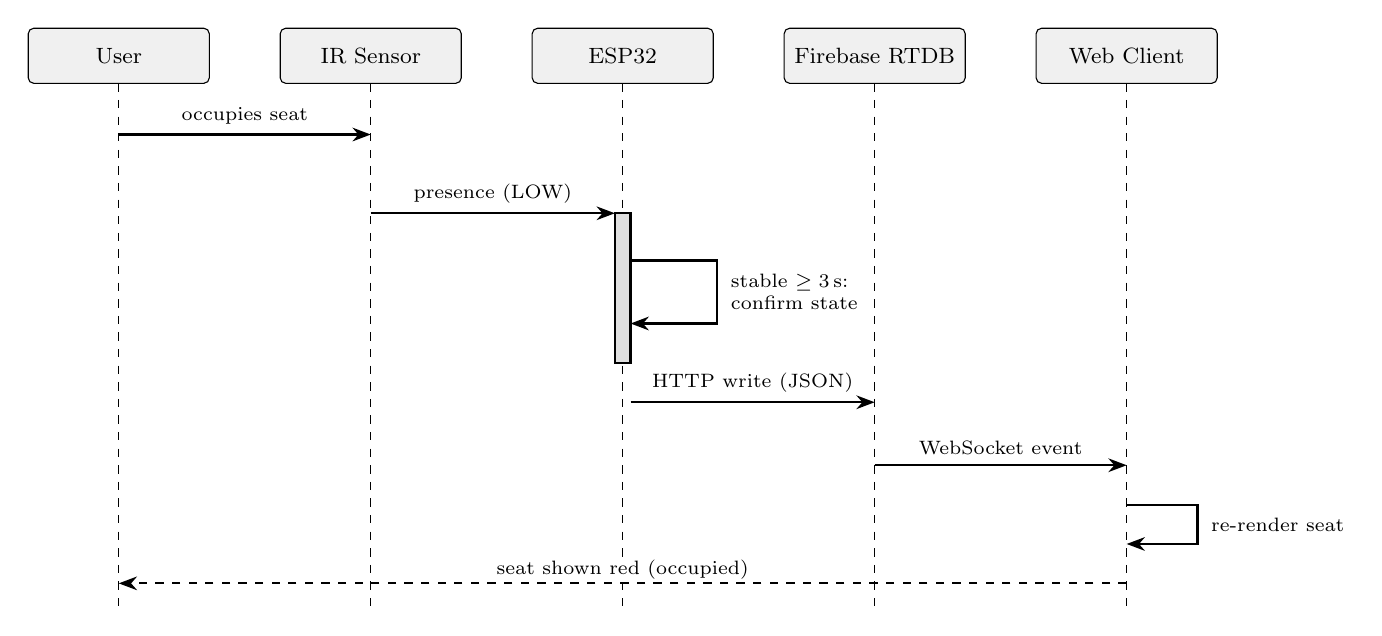
\begin{tikzpicture}[x=1cm,y=1cm]
  \foreach \x/\n in {0/User,3.2/IR Sensor,6.4/ESP32,9.6/Firebase RTDB,12.8/Web Client}{
    \node[draw,fill=gray!12,rounded corners=2pt,minimum width=2.3cm,minimum height=0.7cm,font=\footnotesize] at (\x,0) {\n};
    \draw[dashed] (\x,-0.35) -- (\x,-7.0);
  }
  % activation bar: ESP32 waiting for the debounce window
  \draw[thick,fill=gray!25] (6.3,-2.0) rectangle (6.5,-3.9);
  \draw[->,thick] (0,-1.0)   -- node[above,font=\scriptsize]{occupies seat} (3.2,-1.0);
  \draw[->,thick] (3.2,-2.0) -- node[above,font=\scriptsize]{presence (LOW)} (6.3,-2.0);
  \draw[->,thick] (6.5,-2.6) -- (7.6,-2.6) -- (7.6,-3.4) -- (6.5,-3.4);
  \node[font=\scriptsize,right,align=left] at (7.65,-3.0) {stable $\geq 3$\,s:\\confirm state};
  \draw[->,thick] (6.5,-4.4) -- node[above,font=\scriptsize]{HTTP write (JSON)} (9.6,-4.4);
  \draw[->,thick] (9.6,-5.2) -- node[above,font=\scriptsize]{WebSocket event} (12.8,-5.2);
  \draw[->,thick] (12.8,-5.7) -- (13.7,-5.7) -- (13.7,-6.2) -- (12.8,-6.2);
  \node[font=\scriptsize,right] at (13.75,-5.95) {re-render seat};
  \draw[->,thick,dashed] (12.8,-6.7) -- node[above,font=\scriptsize,fill=white,inner sep=1pt]{seat shown red (occupied)} (0,-6.7);
\end{tikzpicture}}
\caption{Sequence diagram for a seat-occupancy event, including the 3-second debounce}
\label{fig:seq}
\end{figure}

\subsection{Seat State Machine}

Each seat follows the four states in Figure~\ref{fig:fsm}. \textsc{Vacant} and
\textsc{Occupied} are the states sent to the database. In the two \textsc{Pending} states the
firmware waits to see if the new reading holds. If it holds for 3~seconds, the status changes
and is sent. If it changes back sooner (dashed arrows), the seat keeps its old status and
nothing is sent.

\begin{figure}[H]
\centering
\fitfig[0.36]{%
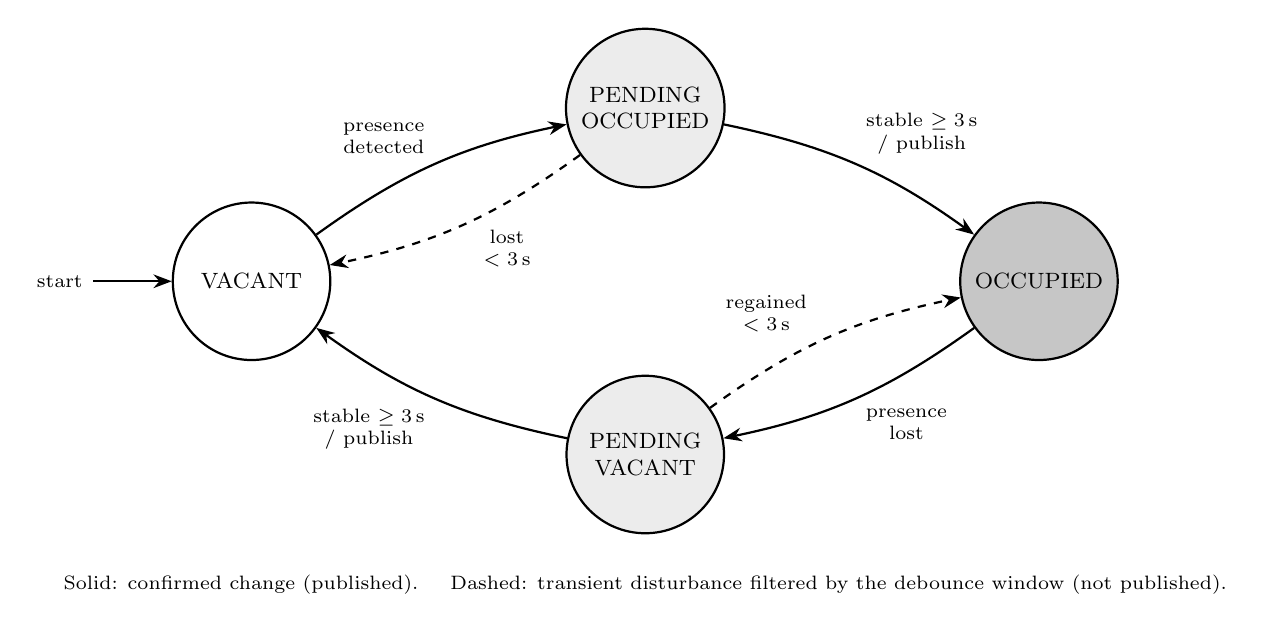
\begin{tikzpicture}[
  st/.style={circle,draw,thick,minimum size=2.0cm,align=center,font=\footnotesize}]
  \node[st,fill=white]   (v)  at (0,0)    {VACANT};
  \node[st,fill=gray!15] (p1) at (5,2.2)  {PENDING\\OCCUPIED};
  \node[st,fill=gray!45] (o)  at (10,0)   {OCCUPIED};
  \node[st,fill=gray!15] (p2) at (5,-2.2) {PENDING\\VACANT};
  \draw[<-,thick] (v.west) -- ++(-1.0,0) node[fl,left]{start};
  \draw[->,thick] (v)  to[bend left=12]  node[fl,above left]{presence\\detected} (p1);
  \draw[->,thick] (p1) to[bend left=12]  node[fl,above right]{stable $\geq 3$\,s\\/ publish} (o);
  \draw[->,thick] (o)  to[bend left=12]  node[fl,below right]{presence\\lost} (p2);
  \draw[->,thick] (p2) to[bend left=12]  node[fl,below left]{stable $\geq 3$\,s\\/ publish} (v);
  \draw[->,thick,dashed] (p1) to[bend left=12] node[fl,below right,pos=0.45]{lost\\$<3$\,s} (v);
  \draw[->,thick,dashed] (p2) to[bend left=12] node[fl,above left,pos=0.45]{regained\\$<3$\,s} (o);
  \node[fl,anchor=north] at (5,-3.6) {Solid: confirmed change (published). \quad
        Dashed: transient disturbance filtered by the debounce window (not published).};
\end{tikzpicture}}
\caption{Seat state machine with 3-second debounce}
\label{fig:fsm}
\end{figure}

\subsection{ESP32 Firmware Flowchart}

Figure~\ref{fig:flow} shows the order of steps in the firmware. After start-up, the loop
reads each sensor, checks whether the reading has changed and held for 3~seconds, and sends
an update only when a seat's status changes. The state machine describes one seat; the
flowchart describes the program.

\begin{figure}[H]
\centering
\fitfig[0.42]{%
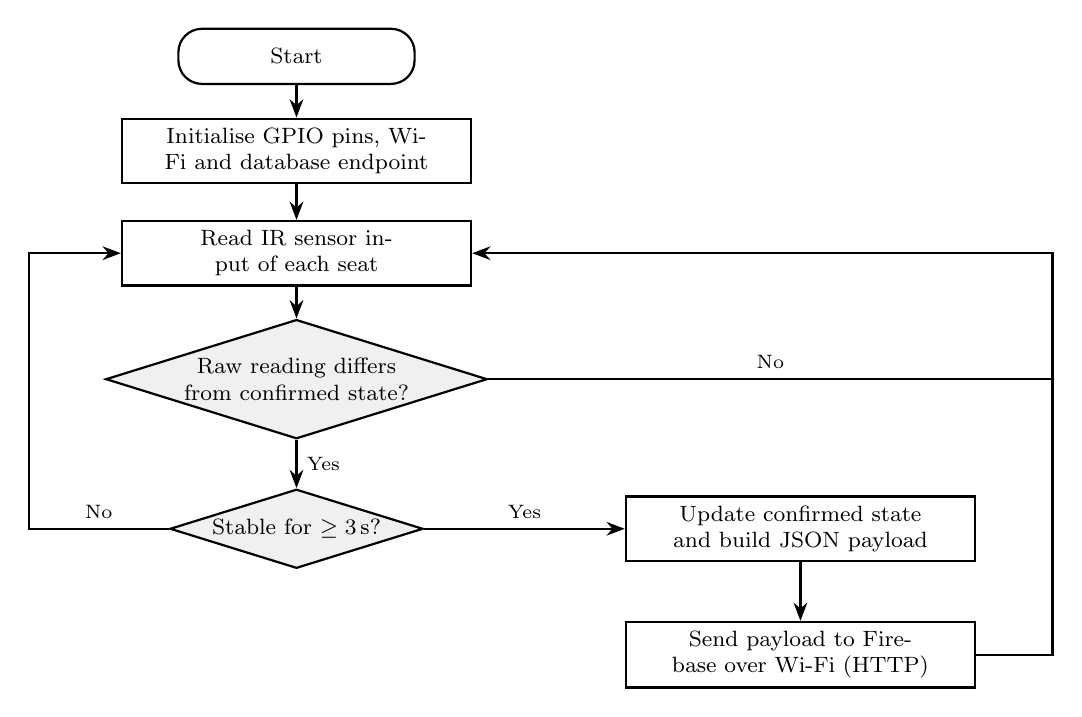
\begin{tikzpicture}[
  term/.style={rectangle,rounded corners=0.3cm,draw,thick,fill=white,minimum height=0.7cm,minimum width=3cm,font=\footnotesize,align=center},
  prc/.style={rectangle,draw,thick,fill=white,minimum height=0.8cm,text width=4.2cm,font=\footnotesize,align=center},
  dec/.style={diamond,aspect=3.2,draw,thick,fill=gray!12,inner sep=1pt,font=\footnotesize,align=center}]
  \node[term] (start) at (0,0)    {Start};
  \node[prc]  (init)  at (0,-1.2) {Initialise GPIO pins, Wi-Fi and database endpoint};
  \node[prc]  (read)  at (0,-2.5) {Read IR sensor input of each seat};
  \node[dec]  (d1)    at (0,-4.1) {Raw reading differs\\from confirmed state?};
  \node[dec]  (d2)    at (0,-6.0) {Stable for $\geq 3$\,s?};
  \node[prc]  (upd)   at (6.4,-6.0) {Update confirmed state and build JSON payload};
  \node[prc]  (send)  at (6.4,-7.6) {Send payload to Firebase over Wi-Fi (HTTP)};
  \draw[->,thick] (start) -- (init);
  \draw[->,thick] (init) -- (read);
  \draw[->,thick] (read) -- (d1);
  \draw[->,thick] (d1) -- node[right,font=\scriptsize]{Yes} (d2);
  \draw[->,thick] (d2) -- node[above,font=\scriptsize]{Yes} (upd);
  \draw[->,thick] (upd) -- (send);
  % loop back to the sensor-reading step (right side)
  \draw[thick] (d1.east) -- node[above,font=\scriptsize]{No} (9.6,-4.1);
  \draw[thick] (send.east) -- (9.6,-7.6) -- (9.6,-4.1);
  \draw[->,thick] (9.6,-4.1) -- (9.6,-2.5) -- (read.east);
  % loop back (left side) when the reading is not yet stable
  \draw[->,thick] (d2.west) -- node[above,font=\scriptsize]{No} (-3.4,-6.0) -- (-3.4,-2.5) -- (read.west);
\end{tikzpicture}}
\caption{Firmware main-loop flowchart}
\label{fig:flow}
\end{figure}

\section{Implementation Details}

\subsection{Firmware (ESP32)}
% (ESP32)}

The firmware reads the IR pins, applies the 3-second debounce to each seat and sends the
confirmed status as JSON. Listing~\ref{lst:fw} shows this logic; pin numbers match
Section~\ref{sec:stack}.

\Needspace{30\baselineskip}
\begin{lstlisting}[style=code,language=C++,caption={Illustrative firmware logic for debounce and publishing},label={lst:fw}]
constexpr uint32_t DEBOUNCE_MS = 3000;   // 3-second debounce window
struct Seat { uint8_t pin; bool confirmed, candidate; uint32_t changedAt; };
Seat seats[2] = { {27, false, false, 0}, {28, false, false, 0} };

void publishState() {                    // build JSON and write once
  String json = "{";
  for (int i = 0; i < 2; ++i) {
    json += "\"s" + String(i + 1) + "\":{\"occupied\":";
    json += seats[i].confirmed ? "true}" : "false}";
    if (i < 1) json += ",";
  }
  json += "}";
  HTTPClient http;  http.begin(DB_URL);
  http.PUT(json);   http.end();          // clients notified by the database
}
void loop() {
  bool dirty = false;
  for (auto &s : seats) {
    bool raw = (digitalRead(s.pin) == LOW);         // active-low IR module
    if (raw != s.candidate) { s.candidate = raw; s.changedAt = millis(); }
    if (s.candidate != s.confirmed && millis() - s.changedAt >= DEBOUNCE_MS) {
      s.confirmed = s.candidate;  dirty = true;
    }
  }
  if (dirty) publishState();
}
\end{lstlisting}

\subsection{Cloud Layer and Web Application}

The Firebase Realtime Database holds the seat status described in Section~\ref{sec:stack}.
The web app listens to the database and receives each change over an open WebSocket
connection, so it never needs to ask for updates.

The web app, called \emph{SmartLib}, is built with React~\cite{react}. It has a
\emph{User} view and an \emph{Admin} view in the navigation bar. Each seat on the map is an
SVG shape whose colour follows its \texttt{occupied} value, so it updates as soon as the
database changes.

\textbf{User dashboard.} Cards show total, taken and free seats and the percentage in use
(for example: 4 seats, 2 taken, 2 free, 50\%). A seat map shows seats S01--S04 around a table,
with free seats in green and taken seats in red.

\textbf{Admin dashboard.} Cards show total seats, taken seats, average session time and the
busiest hour. Charts show the weekly trend, hourly usage and the taken/free split, to help
staff plan.

\textbf{Entrance screen.} The same app shows live seat availability at the library gate.

% ===== CHAPTER 3: RESULTS & EVALUATION =====

\chapter{Results and Evaluation}
\label{ch:results}

\section{Testing Methodology}

The planned tests in Table~\ref{tab:tests} check the requirements from
Chapter~\ref{ch:method}.

\begin{table}[H]
\centering
\small
\renewcommand{\arraystretch}{1.1}
\begin{tabularx}{\linewidth}{|l|>{\raggedright\arraybackslash}p{0.3\linewidth}|>{\raggedright\arraybackslash}X|>{\raggedright\arraybackslash}p{0.19\linewidth}|}
  \hline
  \textbf{ID} & \textbf{Scenario} & \textbf{Expected outcome} & \textbf{Req.} \\
  \hline
  T1 & A person sits in a free seat & After 3\,s the seat turns red on all dashboards
       & FR1, FR2, FR5 \\
  \hline
  T2 & The person leaves the seat & After 3\,s the seat turns green & FR1, FR2, FR5 \\
  \hline
  T3 & A hand or bag passes the sensor for less than 3\,s & No change is sent
       & FR2, NFR2 \\
  \hline
  T4 & Two screens are open at once & Both update together without a refresh
       & FR4 \\
  \hline
  T5 & Seat counts are checked & Taken $+$ free equals total seats; the percentage is
       correct & FR6 \\
  \hline
  T6 & Wi-Fi drops and comes back & The node sends updates again and dashboards show the
       current status & NFR1 \\
  \hline
  T7 & The entrance screen is opened at the gate & It matches the user dashboard
       & FR7 \\
  \hline
  T8 & The admin dashboard is opened & Session time, busiest hour and charts are shown & FR8 \\
  \hline
\end{tabularx}
\caption{Test cases and expected outcomes}
\label{tab:tests}
\end{table}

\section{Analysis}

The prototype shows the full path: IR sensor to ESP32, ESP32 to the cloud database, and
database to live browser dashboards. Sensing each seat fixes the main weakness of gate
counters, and the 3-second debounce keeps seat colours steady.

\subsection{Limitations}

An IR sensor detects any object, not only a person, so a bag left on a desk shows the seat
as taken. The system needs library Wi-Fi and the cloud service, and larger set-ups need more
nodes, careful wiring and power planning, and sensor tuning.

% ===== CHAPTER 4: CONCLUSION =====

\chapter{Conclusion}
\label{ch:concl}

\section{Summary of Work}

This project builds SmartLib, a real-time Library Seat Allocator, from low-cost IoT hardware and a cloud
database. It solves the three problems found earlier: users can see free seats before
walking in, each desk's status is shown instead of a total count, and staff get live and past
usage data.

\section{Future Work and Recommendations}

\begin{enumerate}
  \item Add a second type of sensor to tell a person apart from an object.
  \item Add seat booking with time-limited holds.
  \item Use past data to predict busy hours.
  \item Use a lighter messaging method such as MQTT, and battery or low-power operation.
  \item Cover more zones and floors with a campus-wide map.
  \item Send alerts when a chosen seat or zone becomes free.
\end{enumerate}

% ===== BIBLIOGRAPHY =====

% Entries not cited in the text are still listed
\nocite{pressman,sommerville}

\clearpage
\phantomsection
\addcontentsline{toc}{chapter}{Bibliography}
\begin{thebibliography}{BRJ05}
\bibitem[BRJ05]{uml} Grady Booch, James Rumbaugh, and Ivar Jacobson. \emph{The Unified Modeling Language User Guide}. 2nd ed. Addison-Wesley, 2005.
\bibitem[Esp]{esp32} Espressif Systems. \emph{ESP32 Series Datasheet}. Espressif Systems. \url{https://www.espressif.com}.
\bibitem[Goo]{firebase} Google. \emph{Firebase Realtime Database Documentation}. \url{https://firebase.google.com/docs/database}.
\bibitem[Met]{react} Meta Open Source. \emph{React Documentation}. \url{https://react.dev}.
\bibitem[PM19]{pressman} Roger S. Pressman and Bruce R. Maxim. \emph{Software Engineering: A Practitioner's Approach}. 9th ed. McGraw-Hill, 2019.
\bibitem[Som16]{sommerville} Ian Sommerville. \emph{Software Engineering}. 10th ed. Pearson, 2016.
\end{thebibliography}

\end{document}
